\section{Derivation of closed-loop dynamics}
\begin{frame}
    \frametitle{Outline}
    \tableofcontents[currentsection]
\end{frame}

\begin{frame}
    \frametitle{Derivation of closed-loop dynamics}

    \begin{figure}
        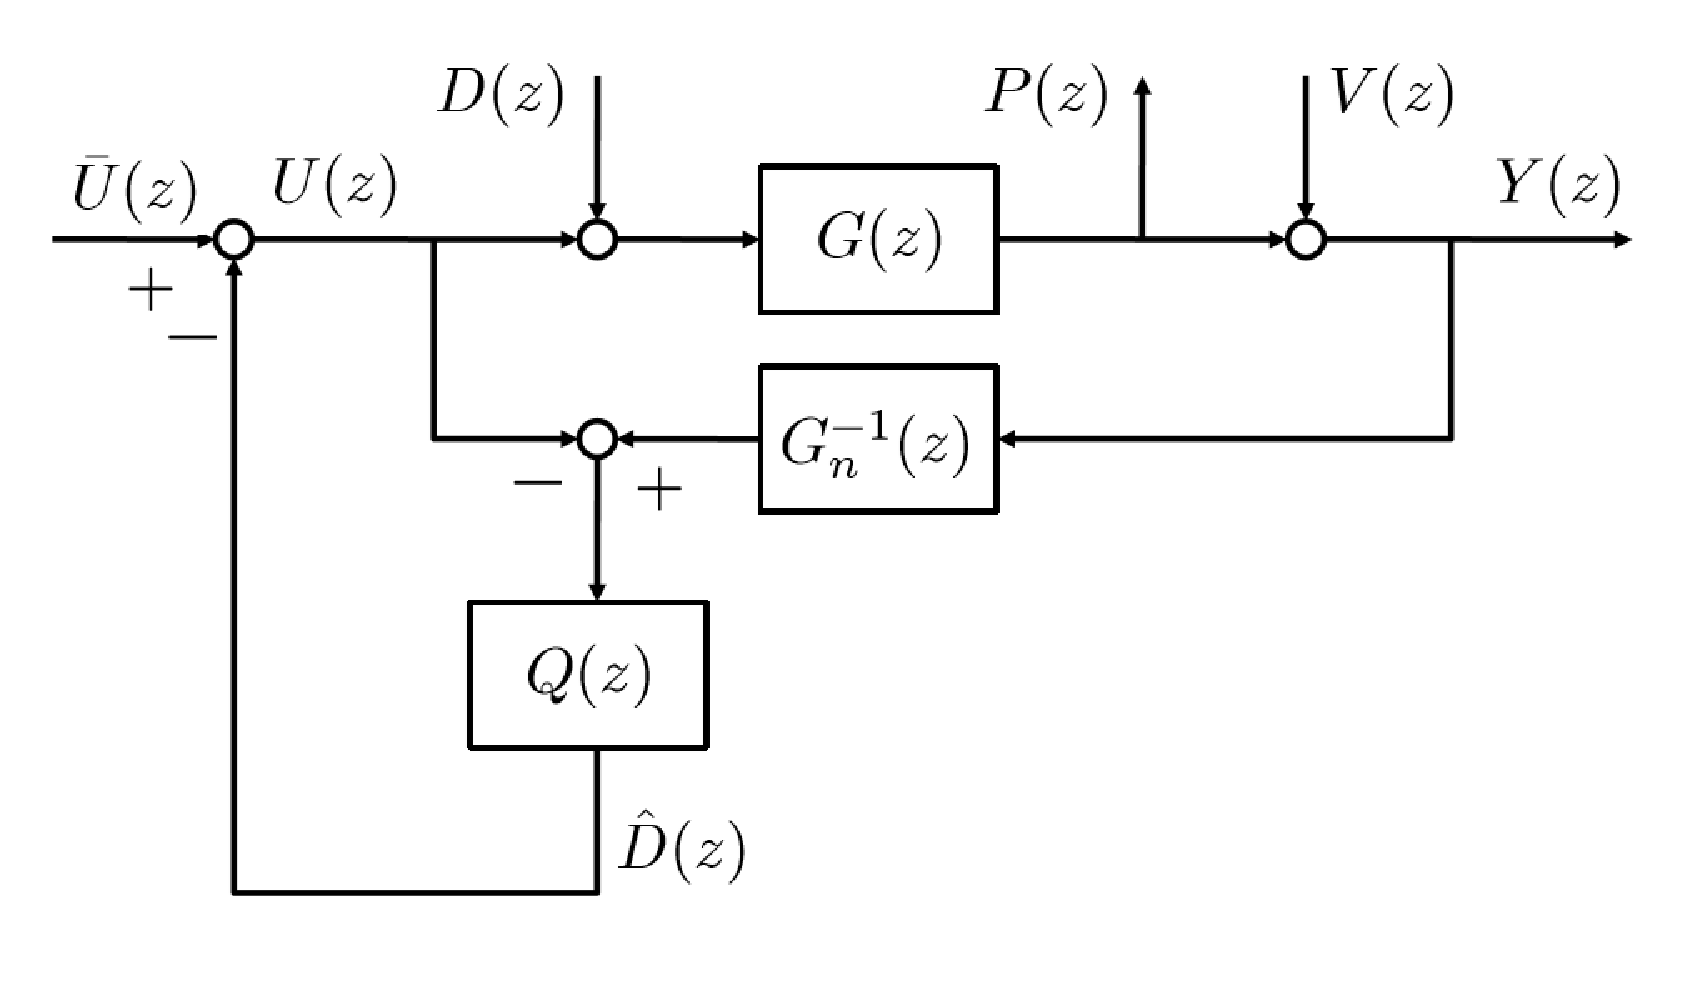
\includegraphics[width=0.5\textwidth]{Disturbance_Observer_DO}\\
    \end{figure}

    We will omit the dependency on $z$ to shorten notation
    \pause

    Plant dynamics: $Y = G(U+D) + V$
    \pause

    Now find the disturbance estimate $\hat{D}$ in terms of $U$, $D$, and $V$:
    \pause
    \begin{gather*}
        \hat{D} = Q (G_n^{-1} Y - U) \\
        \Rightarrow \quad \hat{D} = Q [ G_n^{-1} G (U+D) + G_n^{-1} V - U ] \\
        \Rightarrow \quad \hat{D} = Q ( G_n^{-1} G - 1) U + Q G_n^{-1} GD + QG_n^{-1} V
    \end{gather*}
\end{frame}

\begin{frame}
    \frametitle{Derivation of closed-loop dynamics}

    \begin{figure}
        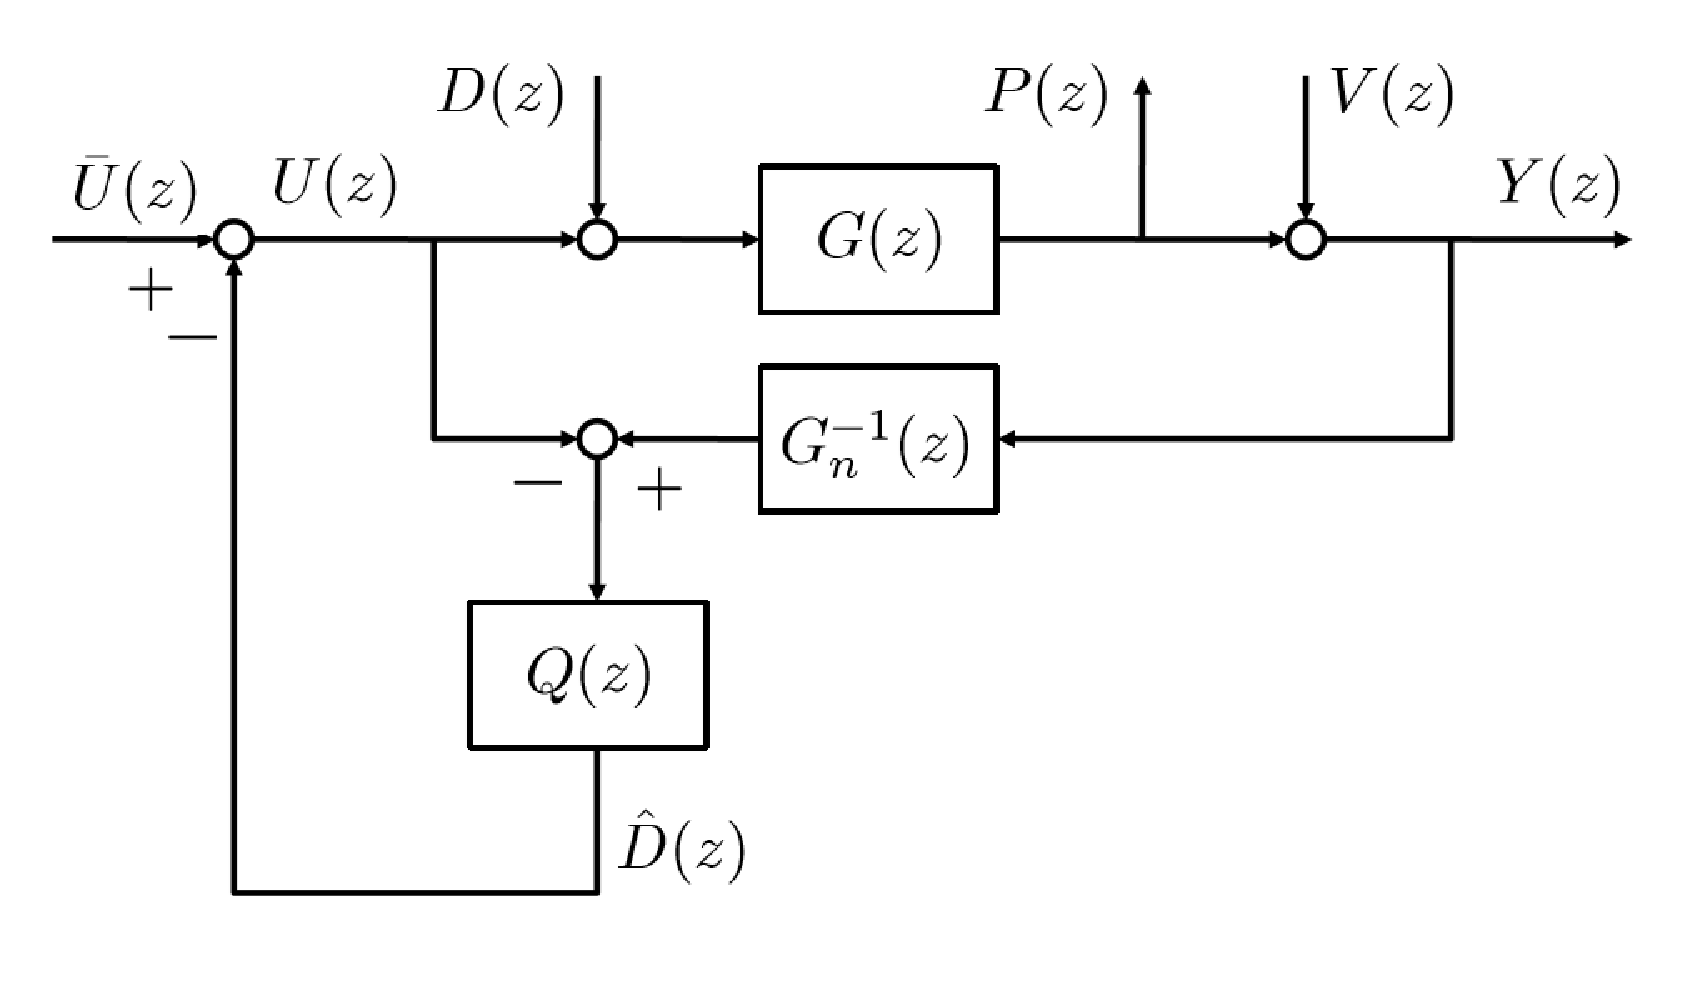
\includegraphics[width=0.5\textwidth]{Disturbance_Observer_DO}\\
    \end{figure}

    Solve for $U$ in terms of $D$, $\bar{U}$, and $V$:
    \begin{gather*}
        U = \bar{U} - \hat{D} \\
        \Rightarrow \quad U = \bar{U} - Q ( G_n^{-1} G - 1) U - Q G_n^{-1} GD - QG_n^{-1} V \\
        \Rightarrow \quad [1 + Q ( G_n^{-1} G - 1)] U = \bar{U} - Q G_n^{-1} GD - QG_n^{-1} V
    \end{gather*}
    \pause
    Now that we have $U$ in terms of $D$, $\bar{U}$, and $V$, we can solve for $P$ in terms of $D$, $\bar{U}$, and $V$
\end{frame}

\begin{frame}
    \frametitle{Derivation of closed-loop dynamics}

    \begin{figure}
        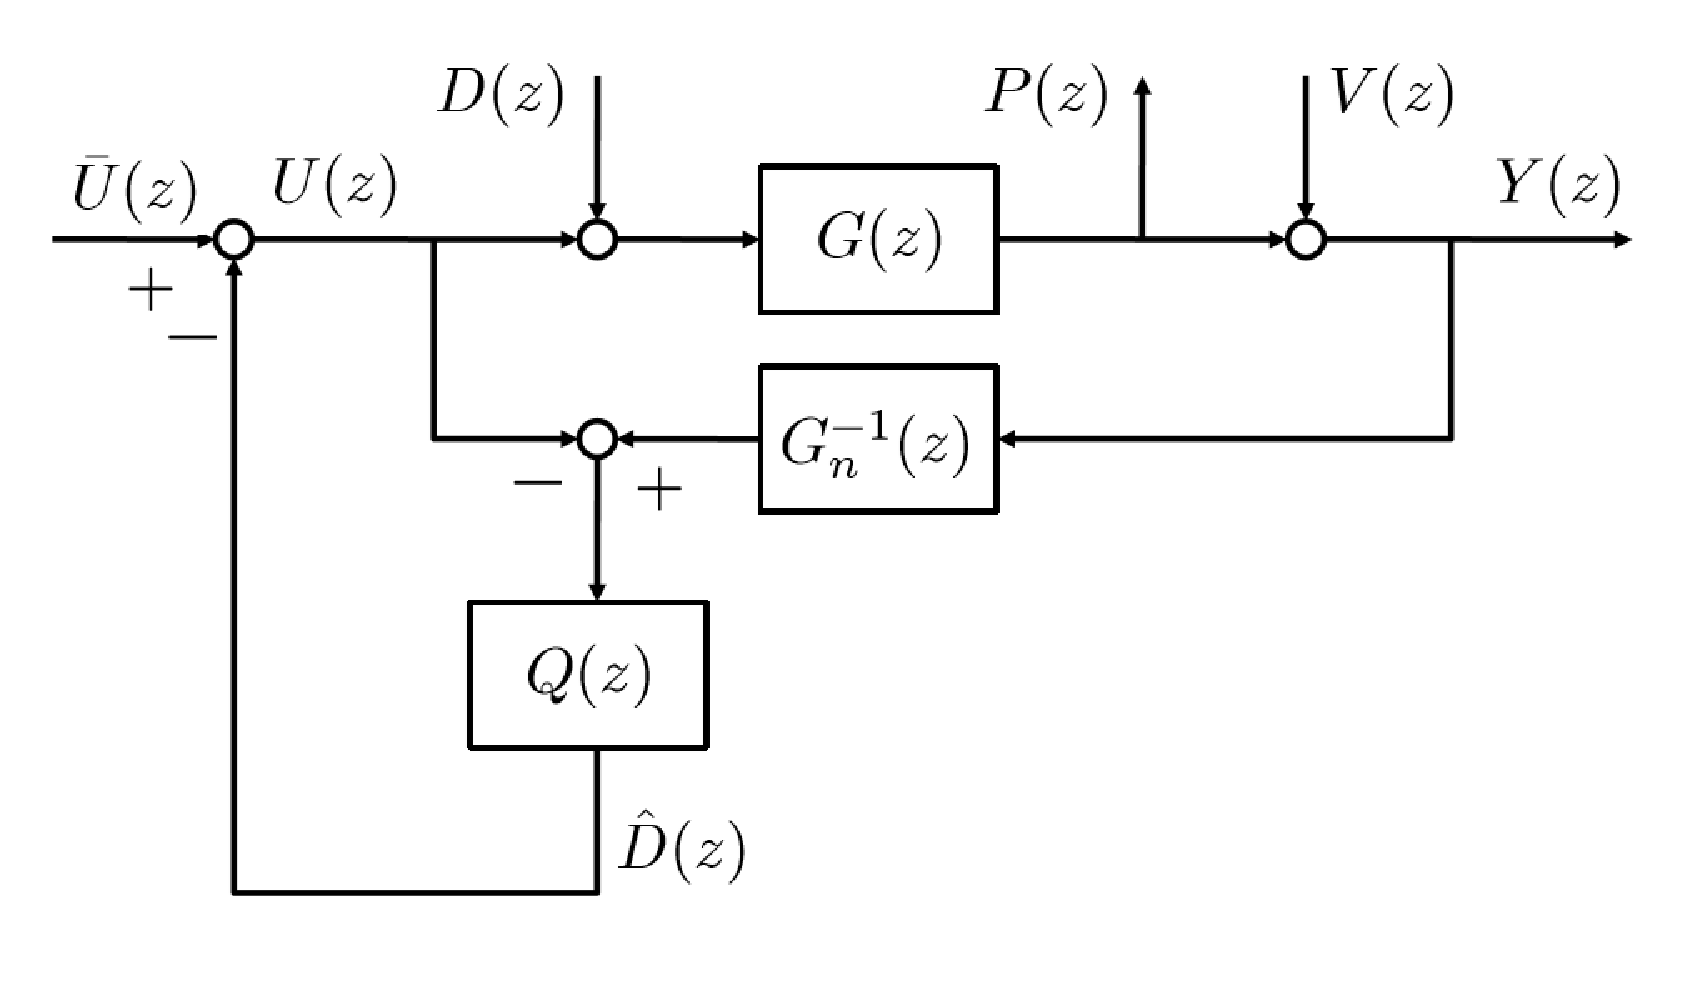
\includegraphics[width=0.3\textwidth]{Disturbance_Observer_DO}\\
    \end{figure}

    Solve for $P$ in terms of $D$, $\bar{U}$, and $V$:
    \begin{gather*}
        P = GD + GU \\
        \Rightarrow \quad P = GD + \frac{G}{1 + Q ( G_n^{-1} G - 1)} 
            [ \bar{U} - Q G_n^{-1} GD - QG_n^{-1} V ]
    \end{gather*}
    \pause
    \alignbox{
        P & = \frac{G (1-Q)}{1 + Q ( G_n^{-1} G - 1)} D + \frac{G}{1 + Q ( G_n^{-1} G - 1)} \bar{U} \\
        & \quad - \frac{GQ G_n^{-1}}{1 + Q ( G_n^{-1} G - 1)} V
    }
\end{frame}

\begin{frame}
    \frametitle{Derivation of closed-loop dynamics}

    \begin{align*}
        P & = \frac{G (1-Q)}{1 + Q ( G_n^{-1} G - 1)} D + \frac{G}{1 + Q ( G_n^{-1} G - 1)} \bar{U} \\
        & \quad - \frac{GQ G_n^{-1}}{1 + Q ( G_n^{-1} G - 1)} V
    \end{align*}

    Let $G(z) = G_n(z) (1 + \Delta(z))$ where $\Delta(z)$ is stable
    \pause

    \alignbox{
        P = \frac{G_n(1+\Delta)(1-Q)}{1+Q \Delta} D + \frac{G_n(1+\Delta)}{1+Q \Delta} \bar{U}
            - \frac{Q(1+\Delta)}{1+Q \Delta} V
    }
    \pause

    In forming this relationship, we used that $G_n G_n^{-1} = 1$, which in turn demonstrates why we require $G_n$ to be minimum phase

\end{frame}


